\documentclass[tikz,border=3mm]{standalone}



\usetikzlibrary{matrix,positioning,fit,backgrounds,intersections}



\begin{document}

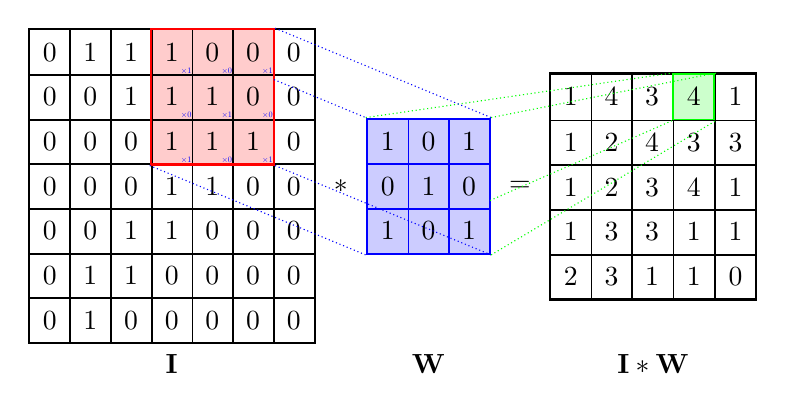
\begin{tikzpicture}[mmat/.style={matrix of math nodes,column sep=-\pgflinewidth/2,
   row sep=-\pgflinewidth/2,cells={nodes={draw,inner sep=5pt,ultra thin}},draw=#1,thick,inner sep=0pt},
   mmat/.default=black,
   node distance=0.3em]
 \matrix[mmat](mat1){
         0 & 1 & 1 & 1 & 0 & 0 & 0 \\ 
         0 & 0 & 1 & 1 & 1 & 0 & 0 \\ 
         0 & 0 & 0 & 1 & 1 & 1 & 0 \\ 
         0 & 0 & 0 & 1 & 1 & 0 & 0 \\ 
         0 & 0 & 1 & 1 & 0 & 0 & 0 \\ 
         0 & 1 & 1 & 0 & 0 & 0 & 0 \\ 
         0 & 1 & 0 & 0 & 0 & 0 & 0 \\ 
         };
 \def\myarray{{1,0,1},{0,1,0},{1,0,1}}       
 \foreach \X in {0,1,2}
 {\foreach \Y in {0,1,2}
  {\pgfmathsetmacro{\myentry}{{\myarray}[\Y][\X]}
  \path (mat1-\the\numexpr\Y+1\relax-\the\numexpr\X+4\relax.south east)
  node[anchor=south east,blue,scale=0.3,inner sep=1.2pt]{$\times\myentry$};
  }}         
 \node[fit=(mat1-1-4)(mat1-3-6),inner sep=0pt,draw,red,thick,name path=fit](f1){};      
 \node[right=of mat1] (mul) {$*$};      
 \matrix[mmat=blue,fill=blue!20,right=of mul,name path=mat2](mat2){    
     1 & 0 & 1 \\ 
     0 & 1 & 0 \\ 
     1 & 0 & 1 \\ };
 \node[right=of mat2] (eq) {$=$};       
 \matrix[mmat,right=of eq](mat3){    
     1 & 4 & 3 & |[draw=green,thick,fill=green!20,alias=4]|4 & 1 \\ 
     1 & 2 & 4 & 3 & 3 \\ 
     1 & 2 & 3 & 4 & 1 \\ 
     1 & 3 & 3 & 1 & 1 \\ 
     2 & 3 & 1 & 1 & 0 \\ 
 };
 \foreach \Anchor in {south west,north west,south east,north east}
 {\path[name path=test] (f1.\Anchor) -- (mat2.\Anchor);
 \draw[blue,densely dotted,name intersections={of=test and fit,total=\t}]
 \ifnum\t>0 (intersection-\t) -- (mat2.\Anchor) \else
  (f1.\Anchor) -- (mat2.\Anchor)\fi;
 \path[name path=test2]  (4.\Anchor) -- (mat2.\Anchor);  
 \draw[green,densely dotted,name intersections={of=test2 and mat2,total=\tt}] 
 \ifnum\tt>0 (intersection-1) -- (4.\Anchor) \else
    (mat2.\Anchor) --  (4.\Anchor)\fi;
    }
 \path (mat1.south) node[below] {$\mathbf{I}$}
  (mat2|-mat1.south) node[below] {$\mathbf{W}$}
  (mat3|-mat1.south) node[below] {$\mathbf{I}*\mathbf{W}$};
 \begin{scope}[on background layer]
  \fill[red!20] (f1.north west) rectangle (f1.south east);
 \end{scope}
\end{tikzpicture}
\end{document}